\documentclass{beamer}

\usefonttheme[onlymath]{serif}
\usepackage[hangul]{kotex}
\usepackage{mathtools}
\usepackage{fancyvrb}
\usepackage{hyperref}
%\input cfrac

\title{mathtools 꾸러미}
\subtitle{amsmath 꾸러미의 확장판}
\author{남수진}
\date{ 2015년 1월 31일\\
2015 한국텍학회 학술대회 및 정기총회 \\
{\small 국가수리과학연구소 (대전)}}

\begin{document}

\begin{frame}
\titlepage
\end{frame}

\begin{frame}[t]
\frametitle{차례}
\tableofcontents
\end{frame}

\section{수식 조판}

\begin{frame}
\huge
\centering 수식 조판
\end{frame}

\begin{frame}
\frametitle{The \TeX book}
\begin{columns}[c]
\column{.5\textwidth}
\textsc{Gentle Reader:}
This is a handbook about \TeX, a new typesetting system intended for the creation of beautiful books---and especially for books that contain \structure{a lot of mathematics.}
\column{.5\textwidth}

\includegraphics[width=2in]{ctan_lion_350x350}
\end{columns}
\end{frame}

\begin{frame}[t]
\frametitle{The \TeX book}
\begin{center} \Large 16, 17, 18, 19, 26, G\end{center}
\begin{align*}
\shortintertext{장(chapter) 수}
\frac{6}{37}&=0.\dot16\dot2\shortintertext{쪽(page) 수}
\frac{120}{483}&=0.\overbrace{\dot24844\ldots2236\dot0}^{66}
\end{align*}

\textbf{16}\quad Typing Math Formulas

\textbf{17}\quad More about Math

\textbf{18}\quad Fine Points of Mathematics Typing
\end{frame}

\section{꾸러미 소개}

\begin{frame}
\huge
\centering 꾸러미 소개
\end{frame}

\begin{frame}[t]
\frametitle{mathtools가 다루는 사항}
\begin{enumerate}
\item \texttt{amsmath} 꾸러미의 버그 수정  
\begin{itemize}
\item \url{http://www.latex-project.org/cgi-bin/ltxbugs2html?
category=AMS+LaTeX}
\item \href{http://www.latex-project.org/cgi-bin/ltxbugs2html?
pr=amslatex/3591&category=AMS+LaTeX}{3591}, \href{http://
www.latex-project.org/cgi-bin/ltxbugs2html?pr=amslatex/
3614&category=AMS+LaTeX}{3614}
\end{itemize}
\item 수식 조판용 유용한 툴 제공 
\begin{itemize}
\item 간단한 매크로 
\item 새로운 수식 환경
\end{itemize}
\end{enumerate}
\end{frame}

\begin{frame}[t]
\frametitle{수식 조판 도구}
\begin{enumerate}
\item \alert{Fine--tuning mathematical layout}
\item Controlling tags
\item Extensible symbols
\item \alert{New mathematical building blocks}
\item Intertext and short intertext
\item \alert{Paired delimiters}
\end{enumerate}
\begin{center}
\texttt{> texdoc mathtools}\\
\href{https://ko.sharelatex.com/blog/2012/06/12/mathtools-for-beautiful-math.html}{Mathtools --- for beautiful math}
\end{center}
\end{frame}

\begin{frame}[fragile]
\frametitle{꾸러미 로딩}
\Large
\alt<2>
{\texttt{\string\usepackage[fleqn,tbtags]\string{\textcolor{red}{mathtools}\string}}}
{\texttt{\string\usepackage[fleqn,tbtags]\string{amsmath\string}}}
\end{frame}


\section{수식 미세 조정}

\begin{frame}
\huge
\centering 수식 미세 조정
\end{frame}

\begin{frame}
\LARGE
\begin{center}
\texttt{\string\mathllap}, 
\texttt{\string\mathclap}, 
\texttt{\string\mathrlap}, \\ 
\texttt{\string\clap}, 
\texttt{\string\mathmbox}, 
\texttt{\string\mathmakebox}, \\ 
\texttt{\string\cramped}, 
\texttt{\string\crampedllap}, \\
\texttt{\string\crampedclap}, 
\texttt{\string\crampedrlap}, \\
\texttt{\string\smashoperator},
\texttt{\string\adjustlimits}
\end{center}
\end{frame}

\begin{frame}
\LARGE
\begin{center}
\textcolor{lightgray}{\texttt{\string\mathllap}}, 
\alert{\texttt{\string\mathclap}}, 
\textcolor{lightgray}{\texttt{\string\mathrlap}}, \\ 
\textcolor{lightgray}{\texttt{\string\clap}}, 
\textcolor{lightgray}{\texttt{\string\mathmbox}}, 
\textcolor{lightgray}{\texttt{\string\mathmakebox}}, \\ 
\textcolor{lightgray}{\texttt{\string\cramped}}, 
\textcolor{lightgray}{\texttt{\string\crampedllap}}, \\
\textcolor{lightgray}{\texttt{\string\crampedclap}}, 
\textcolor{lightgray}{\texttt{\string\crampedrlap}}, \\
\alert{\texttt{\string\smashoperator}},
\alert{\texttt{\string\adjustlimits}}
\end{center}
\end{frame}

\begin{frame}
\frametitle{KTUG QnA 마당}
\url{http://www.ktug.org/xe/index.php?document_srl=158017}

\medskip
\structure{``정렬시 summation과 수식간의 간격 조절에 
대해 궁금합니다.''}

\smallskip
\begin{center}
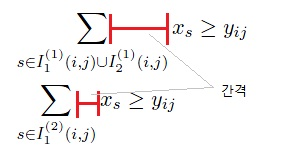
\includegraphics[width=6cm]{mathclap}
\end{center}
\end{frame}

\begin{frame}[fragile]
\frametitle{\texttt{\string\mathclap}}
{\small
\texttt{V = \string\sum\string_\string{\textcolor{red}{s\string\in~I\string_1\string^\string{(1)\string}(i,j)\string\cup~I\string_2\string^\string{(1)\string}(i,j)}\string}x\string_s\string\ge\ y\string_\string{ij\string}}
}
\smallskip
\[
\sum_{ s\in I_1^{(1)}(i,j)\cup I_2^{(1)}(i,j)}x_s\geq y_{ij}
\]

\bigskip
{\small
\texttt{V = \string\sum\string_\string{\textcolor{red}{\string\mathclap\string{s\string\in~I\string_1\string^\string{(1)\string}(i,j)\string\cup~I\string_2\string^\string{(1)\string}(i,j)\string}}\string}x\string_s\string\ge\ y\string_\string{ij\string}}
}
\smallskip
\[
\sum_{\mathclap{s\in I_1^{(1)}(i,j)\cup I_2^{(1)}(i,j)}}x_s\geq y_{ij} 
\]
\end{frame}

\begin{frame}
\frametitle{\texttt{\string\smashoperator}}
\large
\[
\prod_{j\ge0}\biggl(\sum_{k\ge0}a_{jk}z^k\biggr)
  =\sum_{n\ge0}z^n\,\Biggl(\smashoperator[r]{\sum_
       {\scriptstyle k_0,k_1,\ldots\ge0\atop
             \scriptstyle k_0+k_1+\cdots=n}}
    a_{0k_0}a_{1k_1}\ldots\,\Biggr).
\]    
\end{frame}

\begin{frame}[fragile,t]
\frametitle{\texttt{\string\smashoperator}}
\begin{verbatim}
\prod_{j\ge0}\left(\sum_{k\ge0}a_{jk}z^k\right)
  =\sum_{n\ge0}z^n\left(\sum_
       {k_0,k_1,\ldots\ge0\atop k_0+k_1+\cdots=n}
    a_{0k_0}a_{1k_1}\ldots\,\right).
\end{verbatim}
\medskip
\[
\prod_{j\ge0}\left(\sum_{k\ge0}a_{jk}z^k\right)
  =\sum_{n\ge0}z^n\left(\sum_
       {k_0,k_1,\ldots\ge0\atop k_0+k_1+\cdots=n}
    a_{0k_0}a_{1k_1}\ldots\,\right).
\]    
\end{frame}

\begin{frame}[fragile,t]
\frametitle{\texttt{\string\smashoperator}}
\begin{verbatim}
\prod_{j\ge0}\biggl(\sum_{k\ge0}a_{jk}z^k\biggr)
  =\sum_{n\ge0}z^n\,\Biggl(\sum_
     {\substack{k_0,k_1,\ldots\ge0\\ k_0+k_1+\cdots=n}}
    a_{0k_0}a_{1k_1}\ldots\,\Biggr).
\end{verbatim}
\medskip
\[
\prod_{j\ge0}\biggl(\sum_{k\ge0}a_{jk}z^k\biggr)
  =\sum_{n\ge0}z^n\,\Biggl(\sum_
       {\substack{k_0,k_1,\ldots\ge0\\ k_0+k_1+\cdots=n}}
    a_{0k_0}a_{1k_1}\ldots\,\Biggr).
\]    
\end{frame}

\begin{frame}[fragile,t]
\frametitle{\texttt{\string\smashoperator}}
\begin{verbatim}
\prod_{j\ge0}\biggl(\sum_{k\ge0}a_{jk}z^k\biggr)
  =\sum_{n\ge0}z^n\,\Biggl(\sum_{\mathclap
     {\substack{k_0,k_1,\ldots\ge0\\ k_0+k_1+\cdots=n}}}
    a_{0k_0}a_{1k_1}\ldots\,\Biggr).
\end{verbatim}
\medskip
\[
\prod_{j\ge0}\biggl(\sum_{k\ge0}a_{jk}z^k\biggr)
  =\sum_{n\ge0}z^n\,\Biggl(\sum_{\mathclap
       {\substack{k_0,k_1,\ldots\ge0\\ k_0+k_1+\cdots=n}}}
    a_{0k_0}a_{1k_1}\ldots\,\Biggr).
\]  
\end{frame}

\begin{frame}[fragile,t]
\frametitle{\texttt{\string\smashoperator}}
\begin{verbatim}
V = \smashoperator{\sum_{1\le i\le j\le n}}V_{ij}
\end{verbatim}
\[V = \smashoperator{\sum_{1\le i\le j\le n}}V_{ij}\]
\smallskip
\begin{verbatim}
V = \smashoperator[l]{\sum_{1\le i\le j\le n}}V_{ij}
\end{verbatim}
\[V = \smashoperator[l]{\sum_{1\le i\le j\le n}}V_{ij}\]
\smallskip
\begin{verbatim}
V = \smashoperator[r]{\sum_{1\le i\le j\le n}}V_{ij}
\end{verbatim}
\[V = \smashoperator[r]{\sum_{1\le i\le j\le n}}V_{ij}\]
\end{frame}

\begin{frame}[fragile,t]
\frametitle{\texttt{\string\smashoperator}}
\begin{verbatim}
\prod_{j\ge0}\biggl(\sum_{k\ge0}a_{jk}z^k\biggr)
  =\sum_{n\ge0}z^n\,\Biggl(\smashoperator[r]{\sum_
     {\substack{k_0,k_1,\ldots\ge0\\ k_0+k_1+\cdots=n}}}
   a_{0k_0}a_{1k_1}\ldots\,\Biggr).
\end{verbatim}
\medskip
\[
\prod_{j\ge0}\biggl(\sum_{k\ge0}a_{jk}z^k\biggr)
  =\sum_{n\ge0}z^n\,\Biggl(\smashoperator[r]{\sum_
       {\substack{k_0,k_1,\ldots\ge0\\ k_0+k_1+\cdots=n}}}
    a_{0k_0}a_{1k_1}\ldots\,\Biggr).
\]    
\end{frame}

\begin{frame}
\frametitle{\texttt{\string\adjustlimits}}
\Large
\[
\adjustlimits\lim_{n\to\infty} \max_{p\ge n} \quad
\adjustlimits\lim_{n\to\infty} \max_{p^2\ge n} \quad
\adjustlimits\lim_{n\to\infty} \sup_{p^2\ge nK} \quad
\adjustlimits\limsup_{n\to\infty} \max_{p\ge n}
\]
\end{frame}

\begin{frame}[fragile,t]
\frametitle{\texttt{\string\adjustlimits}}
\begin{verbatim}
\lim_{n\to\infty}\max_{p\ge n}
\lim_{n\to\infty}\max_{p^2\ge n} 
\lim_{n\to\infty}\sup_{p^2\ge nK} 
\limsup_{n\to\infty}\max_{p\ge n}
\end{verbatim}
\smallskip
{\Large
\[
\lim_{n\to\infty}\max_{p\ge n} \quad
\lim_{n\to\infty}\max_{p^2\ge n} \quad
\lim_{n\to\infty}\sup_{p^2\ge nK} \quad
\limsup_{n\to\infty}\max_{p\ge n}
\]
}
\end{frame}

\begin{frame}[fragile,t]
\frametitle{\texttt{\string\adjustlimits}}
\begin{verbatim}
\adjustlimits\lim_{n\to\infty}\max_{p\ge n}
\adjustlimits\lim_{n\to\infty}\max_{p^2\ge n} 
\adjustlimits\lim_{n\to\infty}\sup_{p^2\ge nK} 
\adjustlimits\limsup_{n\to\infty}\max_{p\ge n}
\end{verbatim}
\smallskip
{\Large
\[
\adjustlimits\lim_{n\to\infty}\max_{p\ge n} \quad
\adjustlimits\lim_{n\to\infty}\max_{p^2\ge n} \quad
\adjustlimits\lim_{n\to\infty}\sup_{p^2\ge nK} \quad
\adjustlimits\limsup_{n\to\infty}\max_{p\ge n}
\]
}
\end{frame}

\section{새로운 수식 환경}

\begin{frame}
\huge
\centering 새로운 수식 환경
\end{frame}

\begin{frame}[fragile, t]
\frametitle{행렬}
\texttt{\string\matrix*}, 
\texttt{\string\pmatrix*}, 
\texttt{\string\bmatrix*}, 
\texttt{\string\Bmatrix*}, 
\texttt{\string\vmatrix*}, 
\texttt{\string\Vmatrix*}, 

\begin{verbatim}
\begin{matrix*}[<col>]  <contents> \end{matrix*}
\end{verbatim}

옵션인자 col: \alert{c, l, r}

\[
\begin{pmatrix*}
-1&3\\2&-4
\end{pmatrix*}
\quad
\begin{pmatrix*}[l]
-1&3\\2&-4
\end{pmatrix*}
\quad
\begin{pmatrix*}[r]
-1&3\\2&-4
\end{pmatrix*}
\]
\vfill\vfill
\end{frame}

\begin{frame}[fragile]
\frametitle{disallowspaces, allowspaces}
\begin{columns}[c]
\column{1.5in}
\begin{Verbatim*}
\begin{pmatrix*} [r]
-1&3\\
2&-4
\end{pmatrix*}
\end{Verbatim*}
\column{1.5in}
\Large
\[
\begin{pmatrix*} [r]
-1&3\\
2&-4
\end{pmatrix*}
\]
\end{columns}
\end{frame}

\begin{frame}[fragile, t]
\frametitle{disallowspaces, allowspaces}
\begin{verbatim}
\usepackage[allowspaces]{mathtools}
\end{verbatim}

\begin{columns}[c]
\column{1.5in}
\begin{Verbatim*}
\begin{pmatrix*}
[r]&[s]\\
[t]&[u]
\end{pmatrix*}
\end{Verbatim*}
\column{1.5in}
\Large
\[
\begin{pmatrix*}
&[s]\\
[t]&[u]
\end{pmatrix*}
\]
\end{columns}
\end{frame}

\begin{frame}[fragile,t]
\frametitle{case류 환경}
\begin{verbatim}
a= \begin{cases}
      E = mc^2     & Nothing to see here \\
      \int x-3\, dx & Integral is display style
   \end{cases}
\end{verbatim}
\[
a= \begin{cases}
      E = mc^2     & Nothing to see here \\
      \int x-3\, dx & Integral is display style
   \end{cases}
\]
\end{frame}

\begin{frame}[fragile,t]
\frametitle{case류 환경}
\begin{verbatim}
a= \begin{cases*}
      E = mc^2     & Nothing to see here \\
      \int x-3\, dx & Integral is display style
   \end{cases*}
\end{verbatim}
\[
a= \begin{cases*}
      E = mc^2     & Nothing to see here \\
      \int x-3\, dx & Integral is display style
   \end{cases*}
\]
\end{frame}

\begin{frame}[fragile,t]
\frametitle{case류 환경}
\begin{verbatim}
a= \begin{dcases*}
      E = mc^2     & Nothing to see here \\
      \int x-3\, dx & Integral is display style
   \end{dcases*}
\end{verbatim}
\[
a= \begin{dcases*}
      E = mc^2     & Nothing to see here \\
      \int x-3\, dx & Integral is display style
   \end{dcases*}
\]
\end{frame}

\begin{frame}[fragile]
\frametitle{case류 환경}
\Large
\texttt{\string\dcases}, 
\alert{\texttt{\string\dcases*}}, 
\texttt{\string\rcases}, 
\texttt{\string\rcases*}, 
\texttt{\string\drcases}, 
\texttt{\string\drcases*}, 
\texttt{\string\cases*}
\end{frame}

\DeclarePairedDelimiter\abs{\lvert}{\rvert}
\begin{frame}[fragile,t]
\frametitle{Paired delimiters}
\begin{verbatim}
\DeclarePairedDelimiter\abs{\lvert}{\rvert}
\end{verbatim}
\begin{verbatim}
\abs{\frac ab}
\abs*{\frac ab}
\abs[\Bigg]{\frac ab}
\end{verbatim}
\[
\abs{\frac ab} \quad
\abs*{\frac ab} \quad
\abs[\Bigg]{\frac ab}
\]
\end{frame}

\begin{frame}[fragile,t]
\frametitle{왼쪽 윗/아랫첨자}
\begin{verbatim}
{}^{4}_{12}\mathbf{C}^{5+}_{2}          
\prescript{14}{2}{\mathbf{C}}^{5+}_{2} 
\prescript{4}{12}{\mathbf{C}}^{5+}_{2} 
\prescript{14}{}{\mathbf{C}}^{5+}_{2}   
\prescript{}{2}{\mathbf{C}}^{5+}_{2}
\end{verbatim}
{\Large
\[
      {}^{4}_{12}\mathbf{C}^{5+}_{2}          \quad
      \prescript{14}{2}{\mathbf{C}}^{5+}_{2}  \quad
      \prescript{4}{12}{\mathbf{C}}^{5+}_{2}  \quad
      \prescript{14}{}{\mathbf{C}}^{5+}_{2}   \quad
      \prescript{}{2}{\mathbf{C}}^{5+}_{2}
\]}
\end{frame}

\begin{frame}[fragile,t]
\frametitle{Split fractions}
\begin{verbatim}
z=\frac{ab+cd+ef+gh+ij+kl+mn+op+qr}{y}
\end{verbatim}

\[ 
z=\frac{ab+cd+ef+gh+ij+kl+mn+op+qr}{y} 
\]

\begin{verbatim}
z=\frac{\splitfrac{ab+cd+ef+gh+ij}{+kl+mn+op+qr}}{y}
\end{verbatim}

\[
z=\frac{\splitfrac{ab+cd+ef+gh+ij}{+kl+mn+op+qr}}{y}
\]
\end{frame}

\begin{frame}
\huge
\centering 감사합니다.
\end{frame}

\end{document}
